\documentclass[a4paper, 12pt]{article}
\renewcommand{\figurename}{Slika}
%\usepackage[a4paper, total={6in, 8in}]{geometry}
\usepackage[margin=0.5in]{geometry}
\usepackage[T1]{fontenc} %srpski karakteri
\usepackage{graphicx} %figures
\usepackage{caption}
\captionsetup[figure]{font=footnotesize} %the size options for font are: scriptsize, footnotesize, small, normalsize, large, Large

\begin{document}

\title{FV-K2}
\date{Today}
\author{Marko Nikić}
\maketitle
DUV=Design Under Verification
\newpage
\paragraph{Predavanje 8-9 - Strategies for Result Checking}
\paragraph{1 Navesti i ukratko objasniti načine provere ispravnosti rada DUT-a. Uporediti ih međusobno.}
\hfill \break
\indent Yin i yang verifikacije: ne samo da stimulusi moraju dovoljno da istresiraju DUV, već checking komponente moraju da prepoznaju postojanje svih bugova u dizajnu izazvanih ovim stresom. Nakon kreiranja stimulus i checking komponenti, verifikacioni tim može da počne da debaguje DUV i verifikacione komponente. Kada se rezultati DUVa i checking komponente ne slažu, verifikacioni inženjer mora da istraži ovo neslaganje. Ova istraga se naziva \textbf{debug faza}, i tokom ove faze, verifikacioni tim ubira plodove rada izrade komponenti.\\
\indent Tokom faze planiranja verifikacionog testbenča, vođe tima moraju da donesu odluke o generisanju stimulusa (npr. u kom trenutku se stimulusi generišu), koje utiču na results checking deo testbenča.\\
\indent Postoji još jedan apekt results checkinga - u kom trenutku verifikaciono okruženje vrši checking. Postoje dva izbora:
\begin{enumerate}
\item tokom života test slučaja (on-the-fly-checking) ili 
\item na kraju testa (end-of-test checking).
\end{enumerate}
Podsetimo da postoje 3 različita tipa self-checking testbenčeva:
\begin{itemize}
\item Zlatni vektori: Testbenč u kom je određena baza znanja o validnim izlaznim vektorima skladištena u scoreboard-u. Checking komponenta poredi DUV rezultate sa ovom bazom tako što poziva scoreboard i zahteva očekivane vektore. Checker ovo čini ili na svaki ciklus ili na svaku transakciju.
\item Cycle accurate referentni modeli: Testbenč u kom referentni model računa sve očekivane izlaze na osnovu ulaznog stimulusa. Referentni model re-implementira funkciju DUVa, obično u programskom jeziku visokog nivoa (HVL). Checking komponenta poredi izlaze DUVa i referentnog modela.
\item Transaction based: Testbenč u kom DUV ima transakcije koje se mogu identifikovati. Testbenč koristi scoreboard da prati komande i podatke koji se drajvuju na ulaze DUVa. Scoreboard komponenta vrši transformaciju od ulaza do izlaza, i checking komponenta zatim vrši poziv (callback) scoreboard-u kako bi povratila transakciju radi provere.
\end{itemize}
\paragraph{2 Objasniti „On-the-Fly Checking“ pristup provere ispravnosti rada DUT-a. Navesti glavne prednosti ovog pristupa. } 
\hfill \break
\indent On-the-fly checking paradigma znači da verifikaciono okruženje vrši checking tokom simulacije. Stimulus komponente iniciraju transakcije, i kako se ove transakcije završavaju, checking komponente odmah proveravaju njihovu korektnost. Ako checking komponenta detektuje grešku, ona tada zabeleži vreme, transakciju i druge informacije od značaja za debug.\\
\indent Ovaj pristup provere ispravnosti je najprimenjiviji na DUV koji radi sa transakcijama i vrši neku vrstu obrade podataka na toj transakciji. Na slici \ref{img1} je prikazan ovaj tip paradigme.
\begin{figure}[h!]
\centering
%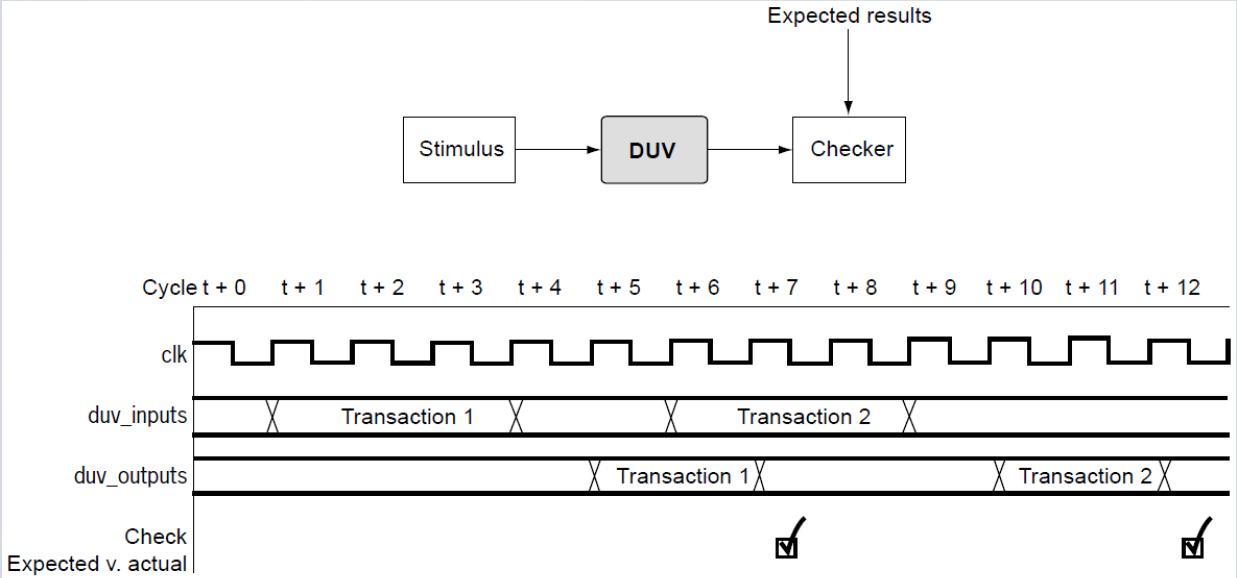
\includegraphics[width=1\textwidth]{img1.png}
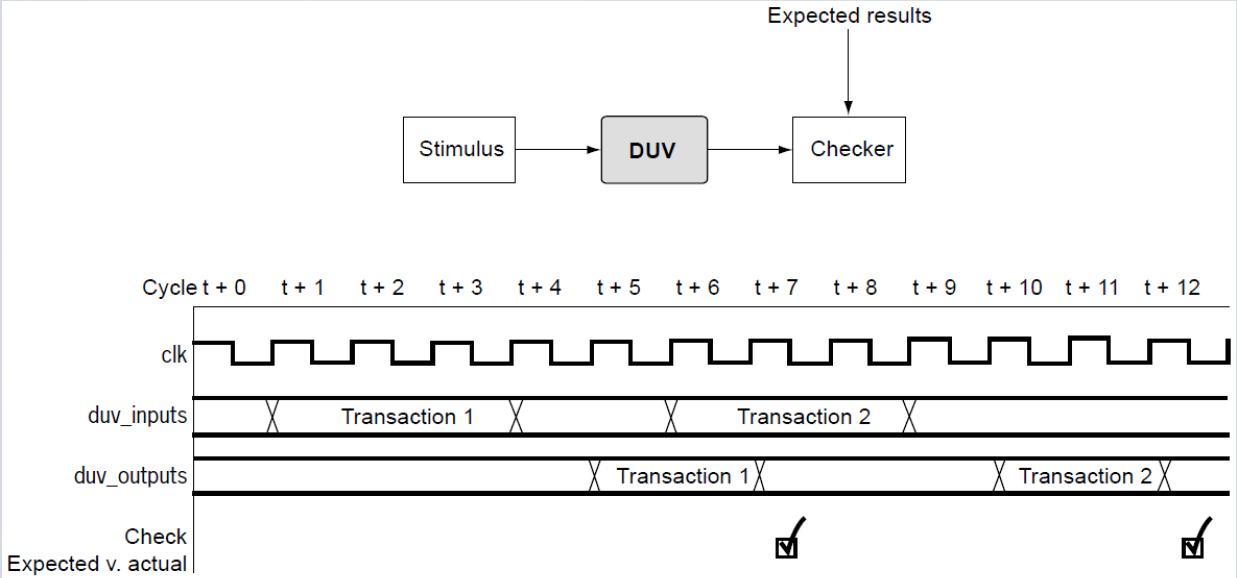
\includegraphics[scale=0.5]{img1.png}
\caption{On-the-fly checking. Stimulus komponenta inicira transakciju koja traje tri ciklusa, u ciklusima t+1 i t+6. Svaka transakcija se završava na izlazima DUVa jedan ciklus nakon kraja transakcije. Checking komponenta oseti kraj izlazne transakcije i u tom trenutku poredi stvarne izlaze sa očekivanim. Ovi očekivani izlazi mogu biti unapred izračunati korišćenjem zlatnih vektora, izračunati od strane scoreboarda kao u transaction-based testbenchu, ili generisani cycle accurate referentnim modelom.}
\label{img1}
\end{figure} 
\\
\indent Postoji više prednosti on-the-fly checking-a:
\begin{itemize}
\item[-]\textbf{Debug} je lakši jer se simulacija zaustavlja kada checker detektuje grešku tokom simulacije, a ne na kraju.
\item[-]Simulacija zahteva \textbf{manje memorije} jer checking komponenta ne mora da zadrži očekivane podatke do kraja simulacije: čim checker završi transakciju, on oslobađa tu memoriju.
\item[-]Pošto je potrebno manje memorije, simulacija se \textbf{izvršava brže} nego u čistom end-of-test checkingu.
\end{itemize}
\paragraph{3 Objasniti „End-of-Test Case Checking“ pristup provere ispravnosti rada DUT-a. Navesti glavne prednosti ovog pristupa.}
\hfill \break
\indent End-of-test Case Checking se primenjuje kada checking komponente treba da provere stanje testbencha nakon završetka simulacionog testa, i to: ili u okviru simulacije (end of simulation checking) ili u odvojenom poslu (post-analysis checking). Koristi se kada je ispunjen jedan od sledećih uslova: \\
- Rezultati ostaju u memoriji DUVa do kraja testa.\\
- Pristup signalima je ograničen (npr. akceleracija ili emulacija).\\
- Zahteva se provera krajnjeg stanja testbencha i/ili DUVa (ispražnjenost redova, poređenje sa referentnim modelom).\\
- Funkcije imaju sistemske aspekte (npr. arbitracija, kašnjenje, performanse).\\
\indent 
Kada se koristi ova checking paradigma, verifikaciono okruženje poziva end-of-test case checking rutinu kada su sve checking komponente odradile svoje. Ova end-of-test rutina će potom izvršiti sve korisnički definisane provere (checks) na testbenchu i DUVu . Slika \ref{img2} ilustruje ovu paradigmu.
\begin{figure}[h!]
\centering
%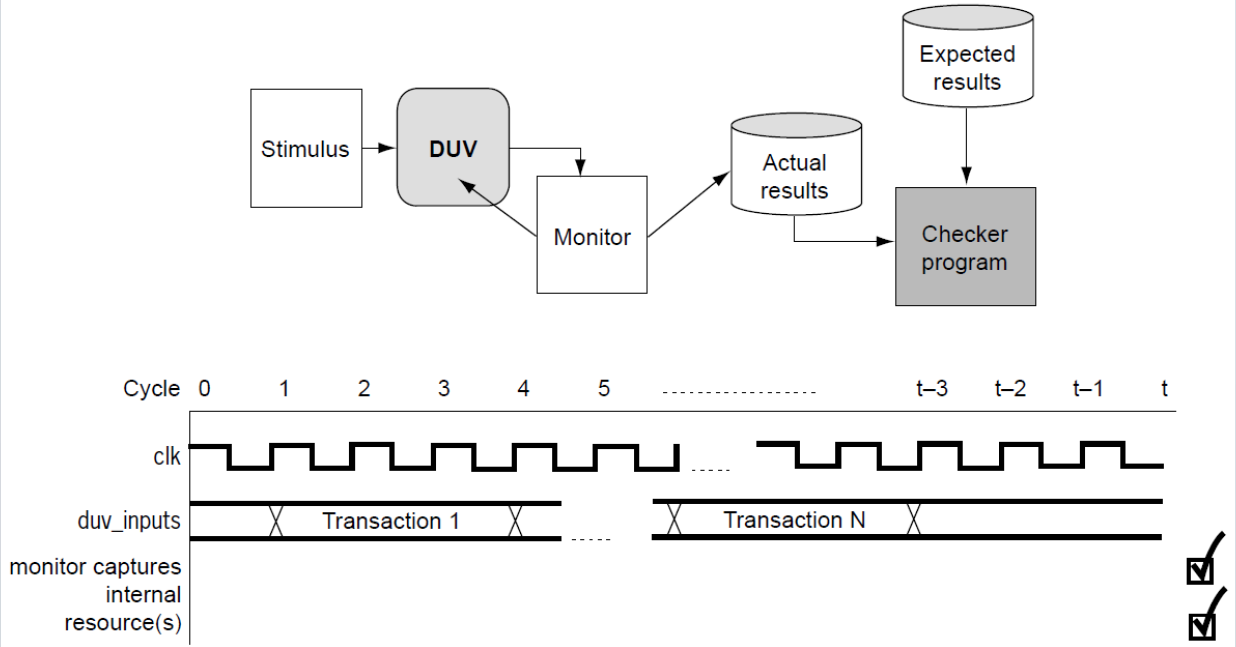
\includegraphics[width=1\textwidth]{img2.png}
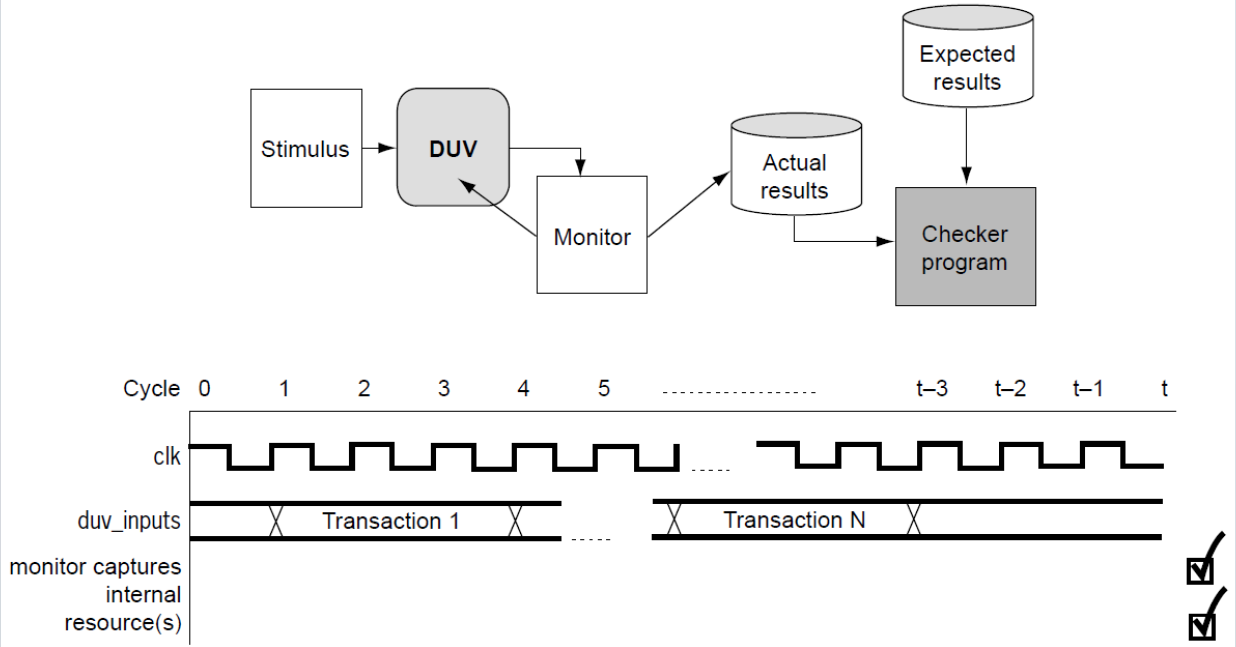
\includegraphics[scale=1]{img2.png}
\caption{End-of-test checking: end of simulation. Stimulus komponenta šalje instrukcije i podatke DUVu tokom simulacije. Monitor nadgleda DUV izlaze tokom simulacije. Kada monitor uoči transakciju na izlazima DUVa, hvata tu transakciju i čuva je u memoriju. (Pored same transakcije, monitor hvata i relevantne podatke i broj ciklusa.) Po završetku simulacije, okruženje poziva checking komponentu, koja validira transakcije uhvaćene od strane monitora tokom test slučaja.}
\label{img2}
\end{figure} 
\\\indent Drugačiji metod za end-of-test case checking je da se provere (checks) vrše izvan simulacionog motora (slika \ref{img3}). Slično je slučaju kada se checking vrši unutar simulacionog engine-a, samo što se ovde simulacioni engine i programi verifikacionog okruženja završe pre nego što odvojeni program započne checking. Monitor sakuplja transakcije na izlazu DUVa, ali umesto u memoriji, upisuje ih u fajl. Kada se simulacija završi, simulacioni program se terminira (na slici se checking ne vrši u simulation wave prozoru). Sada post-processing rutina, nezavisna od simulacionog okruženja, poziva checking koristeći kao ulaze fajlove očekivanih i stvarnih rezultata. Ovaj program proverava ispravnost rezultata.
\begin{figure}[h!]
\centering
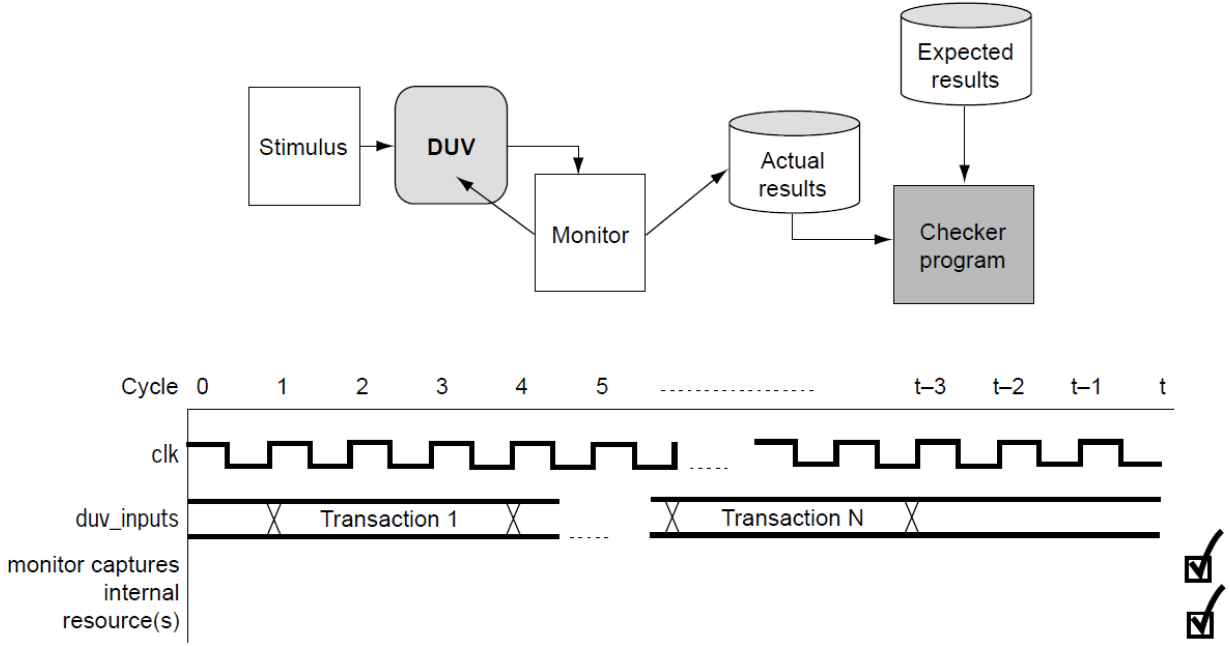
\includegraphics[width=1\textwidth]{img3.png}
\caption{End-of-test checking: postanalysis program. Deo provere rezultata vrši eksterni program koji se poziva nakon što se simulacioni engine završi i terminira.}
\label{img3}
\end{figure} 
\paragraph{4 Objasniti Debug proces prilikom verifikacije dizajna.}
\hfill \break
\indent Debug  je proces lociranja i ispravljanja problema u DUVu ili testbenču. Debug je važan zato što efikasnost ovog procesa štedi vreme i raspored. Mera brzine debuga je brzina kojom verifikacioni tim odredi uzrok neuspeha (failure).\\
\indent Šta se dešava nakon što od checking komponente stigne obaveštenje o neuspehu? Neuspeh može da potekne od bilo kog od postojećih okruženja. Kada test failuje, verifikacioni tim mora da analizira ovaj neuspeh kako bi se našao uzrok problema. Kada test failuje, bug može da postoji u jednom ili više sledećih područja: dizajn, okruženje, specifikacija, alati. Posao verifikacionog inženjera je da pronađe bagove u HDLu i da samo njih prijavi dizajneru. Dakle, verifikacioni inženjer je odgovoran za razvrstavanje neuspeha i razlikovanja dizajn bagova od test bench bagova.\\
\indent Tok debug procesa (debug process flow) počinje u tački neuspeha i prati trag do porekla neuspeha. Slika \ref{img4} ilustruje ovaj proces. Osnovna filozofija iza debug-a je sadržana u pitanju: zašto je test doživeo neuspeh (fail)? Odgovor na ovo pitanje određuje šta popravljamo - HDL, verifikacione komponente, specifikaciju, ili, u retkim slučajevima, alate. Iako ovaj tok deluje jednostavno, kompleksnost debug procesa leži u odlučivanju kojom granom toka poći u blokovima "Expected Data Correct?" i "Inputs Correct?".
\begin{figure}[h!]
\centering
%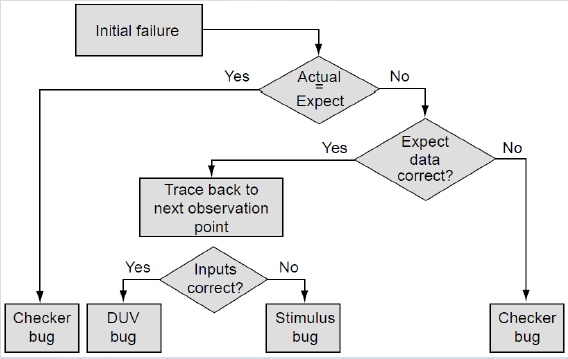
\includegraphics[width=1\textwidth]{img4.png}
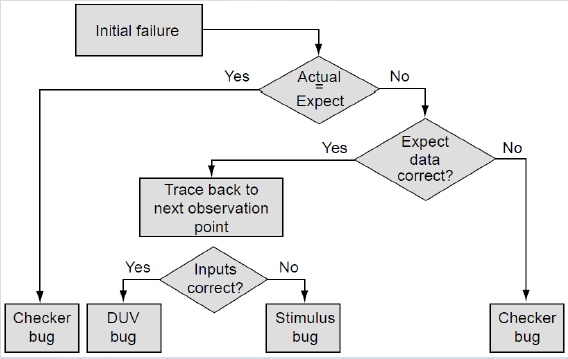
\includegraphics[scale=0.8]{img4.png}
\caption{Debug process flow.}
\label{img4}
\end{figure} 
\\\indent Debug proces određuje neuspeh tako što prati miscompare ili neočekivanu vrednost nazad sve do tačke porekla. Stoga, identifikacija \textbf{tačke neuspeha} (tačke porekla) je kritičan korak. Što je određeni neuspeh bliže \textbf{tački observacije} (checker u kom je okruženje detektovalo miscompare vrednost), to debug proces brže teče. Verifikacioni tim bi mogao da poboljša proces dodavanjem više tačaka observacije za brže izolovanje tačaka neuspeha.\\
\indent Idući u krajnost, svaki čvor u kolu bi mogao da ima check. Međutim, ovo stvara više poteškoća:
\begin{itemize}
\item Prvo, ako verifikacioni tim ugrađuje interne checkove u dizajn, tada se više verifikuje implementacija dizajna (design's implementation) nego namera (design's intent).
\item Drugo, održavanje ekstenzivnih checkera postaje teško, pošto verifikacioni tim mora da updateuje interne checkere sa svakom promenom u dizajnu.
\end{itemize}
\indent Druga krajnost je black box, gde nema tačaka observacije u dizajnu. Ovaj pristup proverava samo izlaze. Međutim, osim ako dizajn nije mali, veoma je verovatno da će tačka neuspeha biti logički udaljena od tačke observacije. Zato se mora balansirati između broja checkera i efikasnosti debuga. "Tačka susreta" ova dva pristupa je gray box paradigma.
\paragraph{5 Tačke observacije (Observation points). Čemu služe i osnovne smernice kojih se treba pridržavati prilikom njihovog postavljanja.}
\hfill \break
\indent Smernice za postavljanje tačaka observacije su:
\begin{itemize}
\item Ciljati na mehanizme definisane u arhitekturi dizajna. Tačke observacije na ovim strukturama su stabilne i zahtevaju manje održavanja.
\item Ravnomerno rasporediti tačke observacije kroz dizajn.
\item Koristiti tačke observacije za uvećanje navoda dizajn tima (design team's assertions). Ne kreirati suvišne tačke observacije za logiku koja već sadrži assertions-e.
\end{itemize}
\paragraph{6 Izveštavanje o detektovanim greškama. Dobar i loš pristup. Ukratko objasniti.}
\hfill \break
\indent Nije dovoljno ukazati na postojanje neuspeha, od podjednakog značaja je i trenutak u kom verifikaciona komponenta prijavi neuspeh. Debug proces ide brže ako checker prijavi neuspeh u trenutku kad se on dogodi. A ako se neuspeh dogodi rano u toku simulacije, ali checking komponenta ukaže na neuspeh tek pri kraju simulacije, pretraga unazad kroz vreme (npr. mnogo transakcija) oduzima mnogo vremena i rasipa simulacione cikluse koji su mogli biti iskorišćeni za druge test slučajeve (test cases). Ovo ukazuje na inherentnu manu end-of-test case checkinga.\\
\indent Na primer, test case se završi i reportuje sledeće:\\
\texttt {Simulation completed:\\
100 transactions sent\\
100 transactions received\\
1 error\\}
\indent Ovaj izveštaj ne pomaže verifikacionom inženjeru u debagovanju, jer ne saopštava kako i kada je checker uočio neuspeh (encountered a failure). Ove poruke nam čak ne govore ni tačku observacije. Ovde bismo neuspeh debugovali pregledanjem trace file-a, ne znajući ni šta je greška bila, ni kada se dogodila.\\
\indent Umesto toga, checker bi trebao da loguje kompletne podatke o neuspehu. To uključuje trenutni ciklus, verifikacioni model, poruku neuspeha, dizajn hijerarhiju u kojoj je checker uočio neuspeh, net-ove uključene u check, stvarne DUV vrednosti i očekivanje vrednosti. Na primer:\\
\texttt{ERROR (Time 50): Checker: Port 1 — Wrong response\\
ERROR (Time 50): Checker: Port 1 — Expected Response: Good\\
ERROR (Time 50): Checker: Port 1 — Actual Response: Overflow\\
ERROR (Time 50): Checker: Port 1 — Expected Result: “0F12023F’’X\\
ERROR (Time 50): Checker: Port 1 — Actual Result: “0F12023E’’X\\}
\indent Posedovanje informacije o načinu i vremenu greške skraćuje vreme debagovnja.
\paragraph{7 Tehnike i alati koji se mogu koristiti u procesu debagovanja. Navesti i objasniti svaki od njih.}
\hfill \break
\indent Razni alati nam pomažu u otkrivanju toga "kako i kada" se dogodio miscompare. Ovi alati postoje kao mehanizmi za smanjenje vremena debagovanja. Kreću se od osnovnih poruka do naprednijih alata koji dozvoljavaju grafički debug test bencha. To su:
\begin{itemize}
\item[-] Print: 
Osnovni mehanizam reportovanja je \textbf{print}. Implementira se dodavanjem print naredbi u komponente okruženja za logovanje test bench aktivnosti. Inženjeri koriste zasebne log fajlove za individualne verifikacione komponente (umesto globalnog log fajla koji bi hvatao poruke svih komponenti), kako bi mogli brže da prođu kroz dosta poruka.\\
Mana je što komponente mogu da generišu hiljade linija poruka u log fajlu. Rešenje je da se u kod okruženja uključe programirani debug nivoi (\textbf{programmed debug levels}). Kada se test case pokreće u default modu, komponente koriste najniži nivo poruka gde checkeri prijavljuju samo greške - ne i dodatne informacije. Ali, kada se dogodi greška, verifikacioni inženjer ponovo pokreće simulaciju, sa višim nivoom debug poruka.
\item[-] Assertions (ne obrađujemo ih)
\item[-] Waveform viewers: 
Kada test case pođe po zlu, često su potrebni dodatni detalji. Verifikacionom inženjeru je potrebno da vidi signale unutar dizajna i njihove vrednosti u različitim trenucima tokom simulacije. Da bi ovo postigao, inženjer koristi waveform viewer. EDA (Electronic design automation) kompanije pružaju ove alate jer je to najčešći tip debugger-a.\\
Waveform vieweri prikazuju signale i lečeve koji su od interesa nakon neuspeha testa i koji, kada se isprate nazad kroz logiku, pomažu da se odredi ispravnost  izlaza. Druga upotreba je da se vidi unutrašnjost debug komponenti. Stimulus, monitor i checking komponente mogu imati interne mašine stanja kao i sam dizajn. 
\item[-] Memory viewers (ne obrađujemo ih)
\end{itemize}
\paragraph{8 Uticaj vrste test bencha na mogućnost efikasnog debug-a.}
\hfill \break
\indent Stimulus i checking paradigme utiču na proces debagovanja. Iako svi tipovi okruženja zahtevaju slične DUV pristupe, različite stimulus i checking tehnike zahtevaju različite pristupe debagovanju samih verifikacionih komponenti. Konkretno, tip generisanja (pre-generation versus on-the-fly generation) i tip checkinga (on-the-fly versus end-of-test case checking) određuju različite interne debug strategije na osnovu informacija dobijenih od test slučaja.\\
\indent Kada se koristi pre-generation strategija, svi objekti (facilities) i stimulusi su dostupni pre pokretanja bilo kog simulacionog ciklusa. Nasuprot tome, on-the-fly generation komponente moraju da pokrenu simulacione cikluse kako bi odlučile da li je stimulus ispravan.
\paragraph{9 Debagovanje unapred generisanih testova.}
\hfill \break
\indent Određivanje ispravnosti stimulusa sa pre-generation stimulus komponentom je lakše i zahteva manje vremena od on-the-fly generisanja. Pre pokretanja bilo kog simulacionog ciklusa, verifikacioni inženjer može da posmatra transakcije koje će stimulus komponenta poslati DUVu. Očekuje se da će stimulus komponenta poslati scenarije u ispravnom formatu. Ako, tokom debugginga, verifikacioni inženjer otkrije da test slučaj sadrži grešku, onda generator (ili writer) mora da popravi problem generisanja. Ako je test slučaj ispravan, ali ulazi u DUV nisu, onda verifikacioni inženjer mora da popravi stimulus komponentu.
\paragraph{10 Debagovanje testova generisanih tokom simulacije.}
\hfill \break
\indent Debagovanje on-the-fly stimulus komponente je sporije nego u pre-generation slučaju. Razlog za to je vreme zaokreta (turn-around time). Verifikacioni inženjer mora da pokrene simulaciju kako bi debug-ovao stimulus komponentu, pa postoji vreme čekanja za određivanje ispravnosti stimulusa. Dodatno, verifikacioni inženjer mora ponovo da pokrene test slučaj i da sačeka da se stigne do iste tačke, kako bi video da li je ispravka bila uspešna.
\paragraph{11 Debagovanje okruženja kod kojih se koristi proveravanje u toku simulacije i na kraju simulacije.}
\hfill \break
\indent Debagovanje end-of-test case i on-the-fly checkinga zahteva slične metode - oba zahtevaju praćenje porekla neuspeha (origin of failure). Stoga je preporučljivo korišćenje debug alata, kao što su print naredbe, u verifikacionom okruženju. Ovi alati dozvoljavaju verifikacionom timu da isprati transakciju od nastanka (generisanja) kroz okruženje do checkera. Često verifikacioni tim dodaje posebna polja strukturama podataka koje se koriste u verifikacionom okruženju. Jedina svrha ovih posebnih polja je da pomognu u praćenju porekla neuspeha.
\paragraph{12 Ponovno korišćenje verifikacionih komponenti (Verification Re-Use). Navesti i ukratko objasniti koje vrste postoje.}
\hfill \break
\indent Re-use omogućava verifikacionom timu da maksimalno iskoristi (to leverage) verifikacione komponente i dizajn blokove na čipu ili na više čipova u sistemu. Kao i za dizajn, i za verifikacione komponente važi koncept "jednom napravi, koristi na više mesta". Rezultat je poboljšano vreme do izbacivanja na tržište (time to market) i smanjeni zahtevi za resursima. Na slici \ref{img6} je primer ponovnog korišćenja dizajna.\\
\begin{figure}[h!]
\centering
%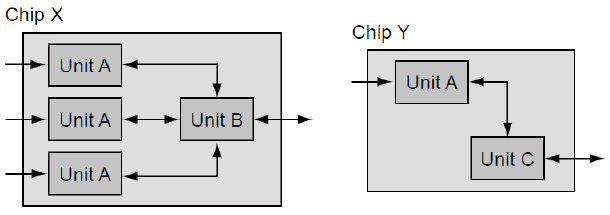
\includegraphics[width=1\textwidth]{img6.png}
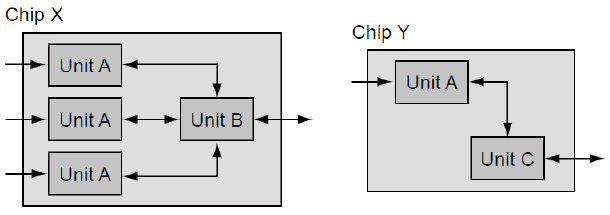
\includegraphics[scale=0.5]{img6.png}
\caption{Design re-use. Višestruka upotreba jednog unit-a (više instanci) na čipu ili na više čipova.}
\label{img6}
\end{figure}
\indent Pošto verifikacija čini veliki deo dizajn napora, ima smisla primeniti na nju koncepte ponovnog korišćenja dizajna. To smanjuje trajanje projekta. Generalno, horizontalni re-use se dešava kada tim koristi dizajn unit ili verifikacionu komponentu na istom nivou hijerarhije. Primer horizontalnog re-usea u verifikaciji dat je na slici \ref{img7}.\\
\begin{figure}[h!]
\centering
%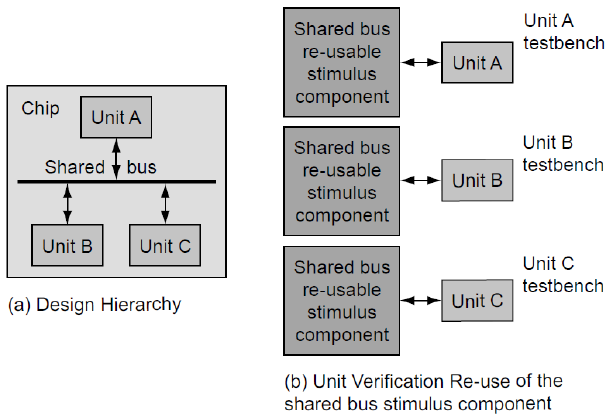
\includegraphics[width=1\textwidth]{img7.png}
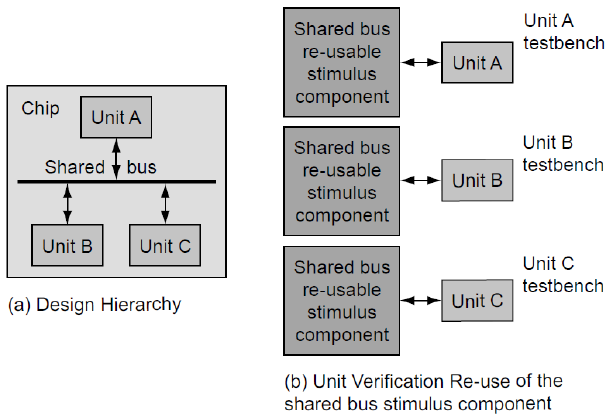
\includegraphics[scale=0.5]{img7.png}
\caption{Horizontal verification re-use: korišćenje verifikacionih komponenti kroz jedan nivo verifikacije. (a) Čip u kom su tri unit-a, A, B, i C, povezani na zajedničku magistralu. (b) Interfejs ka ovoj zajedničkoj magistrali je identičan, tako da verifikacioni tim kreira stimulus komponentu koja se može više puta koristiti za verifikaciona okruženja sva tri unit-a.}
\label{img7}
\end{figure}
\indent Druga forma re-usea, vertikalni re-use, je svojstvena verifikaciji. To je upotreba verifikacionih komponenti kroz više nivoa hijerarhije. Vertikalni re-use je značajan za system simulaciju jer dozvoljava verifikacionom timu da leverage-uje ono što je već implementirano. Ovo, kao i u horizontal re-use slučaju, omogućava optimizaciju resura. Na slici \ref{img8} dat je jednostavan primer vertical verification re-usea.\\
\begin{figure}[h!]
\centering
%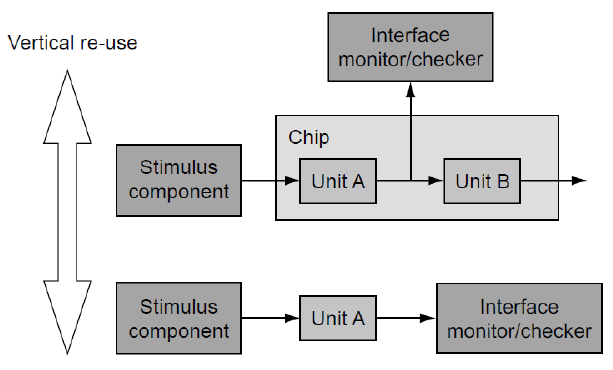
\includegraphics[width=1\textwidth]{img8.png}
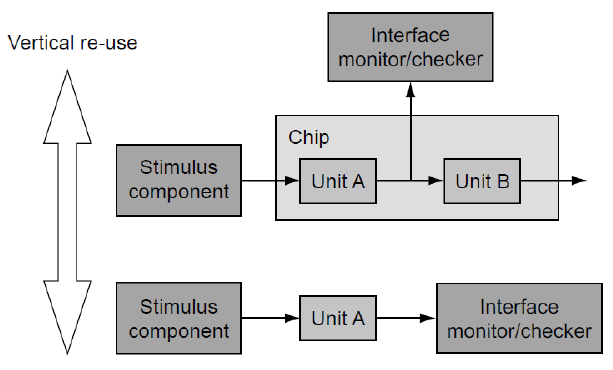
\includegraphics[scale=0.5]{img8.png}
\caption{Vertical verification re-use: korišćenje verifikacionih komponenti kroz razne nivoe hijerarhije (od unit-a do sistema).}
\label{img8}
\end{figure}
\indent Verifikacione komponente koje mogu biti ponovo korišćenje i horizontalno i vertikalno nazivaju se \textbf{re-usable verification IP}. Re-usable verification IP dozvoljava kompanijama da maksimizuju verifikacioni posao. Ovo se dešava ako kompanija razvija više čipova koji koriste interfejs koji je industrijski standard (np. peripheral component interconnect, PCI) i dele stimulus i checking komponente između više projekata.  Kompanije čak mogu i da kupe re-usable verification IP, što im naposletku predstavlja uštedu. 
\paragraph{13 Navesti osnovne smernice kojih se treba pridržavati u cilju kreiranja verifikacionih komponenti koje se mogu ponovo koristiti (re-usable verification components).}
\hfill \break
\indent Re-use deluje lako, ali u stvarnosti par kompanija i grupa postiže visok stepen re-usabilityja, jer ne poštuju smernice kako bi test bench komponente mogle ponovo da se koriste:
\begin{itemize}
\item[-] Nezavisne stimulus komponente
\item[-] Konfigurabilno logovanje poruka
\item[-] Dinamičko mapiranje signala na verifikacione komponente
\item[-] Packaging verifikacionih komponenti
\item[-] Dokumentacija
\end{itemize}
\paragraph{14 Ponovno korišćenje verifikacionih komponenti (Verification Re-Use) - nezavisne stimulus komponente. Objasniti osnovnu ideju.}
\hfill \break
\indent Stimulus komponente moraju da budu nezavisne od ostalih verifikacionih komponenti. Ne bi trebalo da komuniciraju sa bilo kojom drugom komponentom, niti bi bilo koja druga komponenta trebala da komunicira sa stimulus komponentom. Slika \ref{img9} pokazuje zašto su nezavisne stimulus komponente ključne za re-use.
\begin{figure}[h!]
\centering
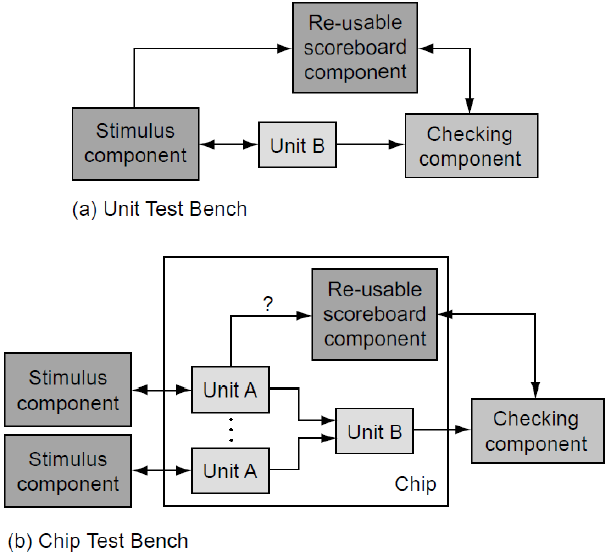
\includegraphics[scale=0.5]{img9.png}
\caption{Nezavisne stimulus komponente. (a) Stimulus komponenta za unit B koja komunicira direktno sa scoreboardom. (b) Upotreba unita B na višem nivou (gde je intermediate checking poželjan za debug); scoreboard sada nije funkcionalan.}
\label{img9}
\end{figure}
\paragraph{15 Ponovno korišćenje verifikacionih komponenti (Verification Re-Use) - dinamičko mapiranje signala. Objasniti osnovnu ideju.}
\hfill \break
\indent Imena interfejs signala kojima monitori, checkeri i stimulus komponente interaguju moraju biti konfigurabilna kako bi se dozvolio horizontalni ili verikalni re-use.\\
\indent U horizontalnom slučaju, jedna verifikaciona komponenta može biti instancionirana više puta u okruženju, ili može biti povezana sa različitim unitima gde svaki unit ima različita imena signala. Calc2 dizajn je dobar primer ovog, prikazano na slici \ref{img10}.\\
\begin{figure}[h!]
\centering
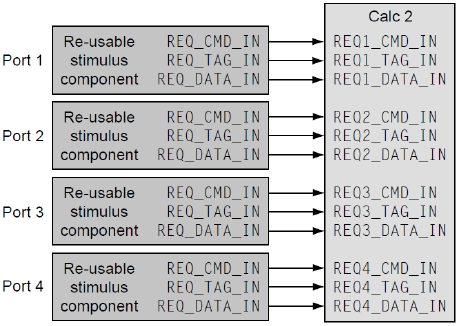
\includegraphics[scale=0.5]{img10.png}
\caption{Horizontal naming issue. Ostavljanjem generičkih imena, ista komponenta se može povezati sa više unita ili sa istim unitom više puta kako bi se olakšao horizontalni re-use.}
\label{img10}
\end{figure}
\indent Kad je vertikalni re-use u pitanju, za mnoga unit okruženja najviši nivo je sam unit. Ipak, kada je unit unutar čipa, postoje dodatni hijerarhijski nivoi. Dakle, verifikacione komponente moraju da budu povezane na različite nivoe. Slika \ref{img11} prikazuje problem vertikalnog imenovanja.
\begin{figure}[h!]
\centering
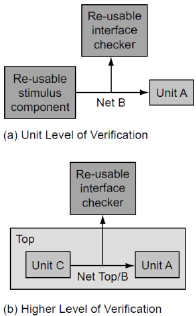
\includegraphics[scale=0.8]{img11.png}
\caption{Vertical naming issue. Ostavljanjem generičkih imena, isti model se može povezati na više nivoa verifikacije kako bi se olakšao horizontalni re-use. (a) Unit level verifikaciono okruženje gde interface checker monitoringuje net B. (b) Isti interface checker je re-useovan ali sada mora da monitoruje Net Top/B.}
\label{img11}
\end{figure}

%----------------------------------------------------------------------------------------------------

\paragraph{Predavanje 10-11 - Monitoring the Verification Flow}
\paragraph{1 Verifikaciona pokrivenost (Verification Coverage). Ukratko objasniti zašto je važna i šta predstavlja.}
\hfill \break
\indent Verifikacionom timu je potrebna metrika kvaliteta i potpunosti njihovog rada kako projekat napreduje tokom vremena. Postoje očigledni kriterijumi potpunosti koje verifikacioni tim može da izvuče iz diskusije verifikacionog plana. Praćenje statusa različitih verifikacionih zadataka je fundamentalna informacija o napredovanju projekta. Znanje o tome koje su testove iz test plana verifikacioni inženjeri zaista izveli nam pruža neophodnu metriku. Praćenje bug rate-a je ključni deo scorekeeping-a koji vodi projekat. I dalje, centralno pitanje je "Kada je verifikacija gotova?". Jednom kada tim završi sve planirane verifikacione zadatke, pokrene sve testove, i bug rate padne na nulu, da li tada verifikaciju možemo proglasiti uspešnom?\\
\indent Iscrpna simulacija čak i malih dizajnova nije moguća. Sledeći primer ukazuje na kombinatornu eksploziju koja čini verifikaciju nezgodnim zadatkom. Neka je DUV 16-bitni sabirač. Simuliranje svih kombinatornih mogućnosti ovog sabirača traje 4 milijarde simulacionih ciklusa, pretpostavljajući da kolo nema elemente za čuvanje stanja. Ako projekat koristi simulacioni engine koji može da pokrene 1000 ciklusa u sekundi, timu će i dalje biti potrebno oko 50 dana da iscrpno simulira ovaj trivijalni DUV. \\
\indent Kada verifikacioni tim zaustavlja simulaciju? Da li je dovoljno nastaviti dok simulacija nije imala bagova 3 dana? Kako da znamo da još jedan dan simulacije ne bi doneo novi bug? Da li je zaista neophodno iscrpno simulirati sabirač kako bi se uverljivo pokazala potpunost verifikacije?\\
\indent Upravo \textbf{analiza verifikacione pokrivenosti} (verification coverage analysis) ima za zadatak da uveri verifikacioni tim da su \textbf{dovoljno}, ne iscrpno, verifikovali, i da su zadovoljili definisane kriterijume kvaliteta. Verifikaciona pokrivenost je mera prostora stanja koju je verifikacija bazirana na simulaciji dotakla u čitavom okruženju. Pokrivenost može da meri interna stanja DUVa, redove, i aktivnosti, kao i DUV ulaze, čak i stanja komponenti verifikacionog okruženja. U osnovi, pokrivenost je mera toga koliko su \textbf{dobro} stimulus komponente izupotrebljavale DUV. Pokrivenost ne može da oceni kvalitet ili robusnost checking komponenti.
\paragraph{2 Oblasti unutar verifikacionog okruženja gde se može meriti verifikaciona pokrivenost (Verification Coverage Target Areas).}
\hfill \break
\indent Postoje dve potpuno komplementarne strane verifikacione pokrivenosti.\\
\indent Prvo, tu je pokrivenost verifikacionog okruženja. Ovde je cilj izmeriti koliko dobro verifikaciono stimulus okruženje pokriva specifikaciju dizajna. Ovaj aspekt pokrivenost naziva se pokrivenost verifikacionog testa (\textbf{verification test coverage}).\\
\indent Drugo, postoji pokrivenost funkcije implementirane DUVom. Ova metrika meri koliko dobro verifikacioni stimulus aktivira ili upotrebljava (exercise) implementaciju specifikacije u konkretnom dizajnu. Ovaj zadatak pokrivenosti se naziva pokrivenost implementacije (\textbf{coverage implementation}). Slika \ref{img-p10-1} pokazuje dve oblasti analize pokrivenosti, jednu pored druge.
\begin{figure}[h!]
\centering
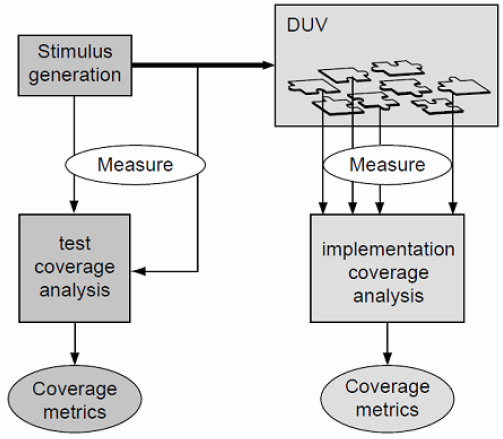
\includegraphics[scale=0.6]{img-p10-1.png}
\caption{Verification Coverage Target Areas.}
\label{img-p10-1}
\end{figure}
\\ \indent Osnovna aktivnost koja prethodi bilo kakvoj analizi pokrivenosti je sakupljanje merenja pokrivenosti (coverage measurements). Verifikacioni tim sakuplja merenja za \textbf{test coverage} od komponente koja inicira stimuluse, test slučaja, ili interfejsa u DUV. \textbf{Implementation coverage} analiza se oslanja na merenja aktivnosti unutar DUVa, koja se dobijaju pregledom HDL modela tokom simulacije.\\
\indent Kroz aktivnosti merenja i analize, verifikacioni tim ne sme da zaboravi da je krajnji cilj analize pokrivenosti da usmerava verifikacioni proces, a ne da dokazuje njegovu potpunost. Potpunost je nedostižan cilj.
\paragraph{3 Ciljevi merenja verifikacione pokrivenosti (Verification Coverage Goals).}
\hfill \break
\indent Naizgled jednostavan cilj pokrivenosti bio bi kombinatorni prostor obuhvaćen enumeracijom svih mogućih šablona na DUV ulazima, svih mogućih internih stanja DUVa i svih izlaznih šablona na izlazima DUVa. Ova metrika je trivijalna, ali i beskorisna, jer se ne može postići.\\
\indent Analiza pokrivenosti bi se mogla definisati kao maksimizovanje \textbf{verovatnoće stimulisanja i detektovanja bugova}, sa minimalnim troškovima (po pitanju vremena, rada i računanja). Detekcija skrivenih bugova jeste glavni cilj verifikacionog procesa.\\
\indent Slika \ref{img-p10-2} ilustruje kako informacije o pokrivenosti mogu da usmeravaju simulaciju kroz prostor stanja DUVa kako bi se pronašli skriveni bugovi. Generisani stimulusi drajvuju simulaciju krivudavim putem kroz prostor stanja. Pokrivenost treba da navodi simulaciju na oblasti koje potencijalno sadrže bugove (sklone su bugovima). Količina skrivenih bugova koje otkrijemo je mera kvaliteta analize pokrivenosti.\\
\indent Pokrivenost je alat koji pomaže verifikacionom timu u pronalaženju bugova, ali je ona samo sredstvo za postizanje cilja. Mera pokrivenosti koja se postigne bez pronalažena bugova ima ograničenu vrednost. Nemoguće je simulacijom pokriti sve delove dizajna. Dakle, pokrivenost mora da se foksira na oblasti sklone greškama. U ovom smislu dobra metrika pokrivenosti mora da ima prediktivnu komponentu; mora da bude sposobna da meri pokrivenost bugova (\textbf{bug coverage}).\\
\begin{figure}[h!]
\centering
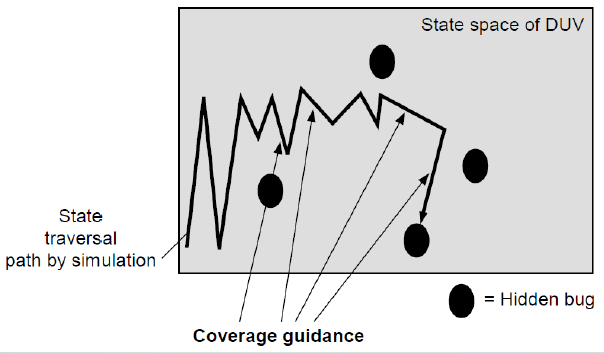
\includegraphics[scale=0.6]{img-p10-2.png}
\caption{Verification coverage guidance to the hidden bugs. Simulacija prolazi kroz prostor stanja DUVa duž cik-cak putanje. Skriveni bugovi su prikazani kao zatamnjeni krugovi. Uticaj navođenja pokrivenosti je prikazan strelicama koje uzrokuju promenu pravca simulacije, nadamo se ka skrivenim bugovima.}
\label{img-p10-2}
\end{figure}
\paragraph{4 Navesti i ukratko objasniti vrste modela verifikacione pokrivenosti koji se koriste u praksi.}
\hfill \break
\indent Slika \ref{img-p10-1} razlikuje pokrivenosti po njihovim ciljnim oblastima- test coverage versus implementation coverage. Postoje razne šeme za specifikaciju metrika pokrivenosti za obe oblasti. Ove šeme nazivaju se \textbf{modelima pokrivenosti}.\\
\indent Moguće je klasifikovati modele pokrivenosti na \textbf{strukturne(code)} i \textbf{funkcionalne}. Obe klase se primenjuju na pokrivenost verifikacionog testa ili pokrivenost implementacije. \textbf{Funkcionalni modeli pokrivenosti} se fokusiraju na \textbf{semantiku} testa ili dizajn-implementacije. Npr. da li je test pokrio sve moguće komande ili da li je simulacija ikada trigerovala overflow FIFO bafera? \textbf{Strukturni (code) modeli pokrivenosti} se vezuju u reprezentaciju domena koji se pokriva. Dobar primer strukturnog modela pokrivenosti je \textbf{line coverage}, mera toga da li su tokom simulacije posećene sve linije source koda u programu stimulus generatora ili HDLu DUVa.
\paragraph{5 Strukturna pokrivenost (Code Coverage). Osnovna ideja, dobre I lose strane. Navesti i ukratko objasniti najcešće korišćene mere.}
\hfill \break
\indent Primena strukturnih modela pokrivenosti je većinom analiza pokrivenosti implementacije. Ovi modeli se uvek vezuju za strukturni aspekt implementacije generisanja testa, DUVa ili reprezentacije dizajn HDLa. Obradićemo najčešće mere strukturne pokrivenosti: toggle, line, statement, branch, path, condition i FSM coverage.
\paragraph{6 Toggle coverage.}
\hfill \break
\indent Toggle coverage meri koliko su puta tokom simulacije signali i lečevi u HDL modelu promenili svoju logičku vrednost. Odsustvo promene signala u delu DUVa ukazuje na to da stimulusi uopšte ne targetiraju ovu oblast. Prednost toogle pokrivenosti je što je u pitanju jednostavan model lak za razumevanje. Mana je, ipak, što ovaj model proizvodi masivne količine podataka, i činjenica da su se svi signali u DUVu toglovali ne pruža nam nikakav uvid u funkcionalni značaj urađenog testinga. Primer toggle pokrivenosti za 11-bitni reg signal prikazan je na slici \ref{img-p10-3}. Neki alati za code coverage prijavljuju ne samo tranzicije sa 0 na 1 i obrnuto, već i tranzicije sa i na nedefinisanu ("X") i tristate ("Z") vrednost.
\begin{figure}[h!]
\centering
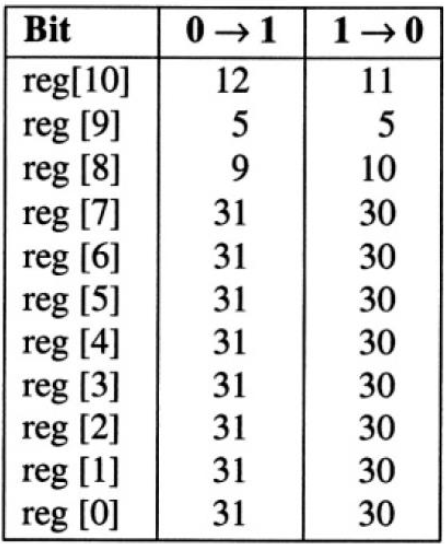
\includegraphics[scale=0.4]{img-p10-3.png}
\caption{Toggle Coverage Example.}
\label{img-p10-3}
\end{figure}
\paragraph{7 Line coverage.}
\hfill \break
\indent Line coverage uzima sintaksnu strukturu HDL specifikacije i meri koje HDL linije su izvršene u simulaciji. Slično toggle pokrivenosti, ovaj model pokrivenosti je lak za razumeti, i odsustvo aktivnosti u delovima HDL modela ukazuje na propuste u testovima. Ograničenje line pokrivenosti je to što nam nedostaje semantički uvid. Činjenica da se HDL naredba (statement) izvršila nam ne govori ništa o ispravnosti sadržaja naredbe. Primer je dat na slici \ref{img-p10-4}.
\begin{figure}[h!]
\centering
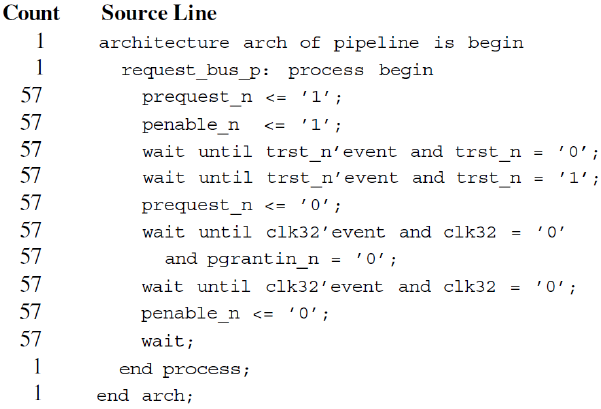
\includegraphics[scale=0.5]{img-p10-4.png}
\caption{Line Coverage Example.}
\label{img-p10-4}
\end{figure}
\paragraph{8 Statement coverage.}
\hfill \break
\indent Statement coverage izveštava o tome koje RTL naredbe su se izvršile, a koje nisu. Ova metrika je preciznija od line pokrivenosti jer naredbe mogu da obuhvataju više linija i više od jedne naredbe može da se nalazi u jednoj liniji. Primer na slici \ref{img-p10-5}.
\begin{figure}[h!]
\centering
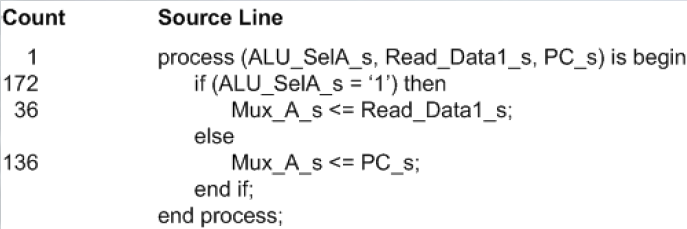
\includegraphics[scale=0.5]{img-p10-5.png}
\caption{Statement Coverage Example.}
\label{img-p10-5}
\end{figure}
\paragraph{9 Branch coverage.}
\hfill \break
\indent Branch coverage ili uslovni coverage pregleda uslovne naredbe (if, case, while, repeat, forever, for i loop) u HDLu i prati koje od ovih uslova simulacija susretne, a koje ne. Ovaj model pretpostavlja da postoji semantičko značenje u uslovima koje je dizajner izrazio u HDLu. Tačke odluke u HDL specifikaciji obično predstavljaju različite uslove na koje dizajn treba da odreaguje. Zato, odsustvo donošenja odluka na sve moguće, predviđene načine ukazuje na nedostatak testinga. Primer na slici \ref{img-p10-6}.
\begin{figure}[h!]
\centering
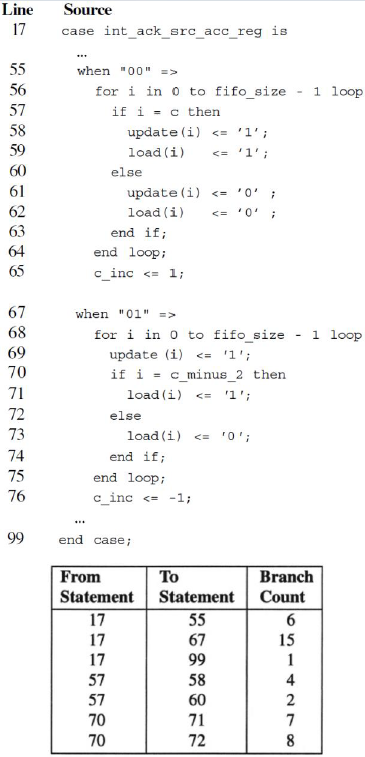
\includegraphics[scale=0.6]{img-p10-6.png}
\caption{Branch Coverage Example.}
\label{img-p10-6}
\end{figure}
\paragraph{10 Path coverage.}
\hfill \break
\indent Path coverage je profinjenje branch coverage-a. Path pokrivenost izveštava o tome koliko je puta svaka moguća putanja u kodu izvršena. Umesto posmatranja jedne uslovne odluke zasebno, path pokrivenost analizira tok izvršavanja HDLa i grupiše kombinacije odluka u putanje izvršavanja. Slika \ref{img-p10-7} pokazuje automatsko generisanje četiri moguće putanje izvršavanja na datom HDLu sa if/then/else strukturom. Da je branch pokrivenost korišćena, ukazala bi da je prođeno svim granama. Ali samo path pokrivenost može otkriti da jednom od mogućih putanja kroz strukturu nije prođeno, što je značajna indikacija za verifikacioni tim.
\begin{figure}[h!]
\centering
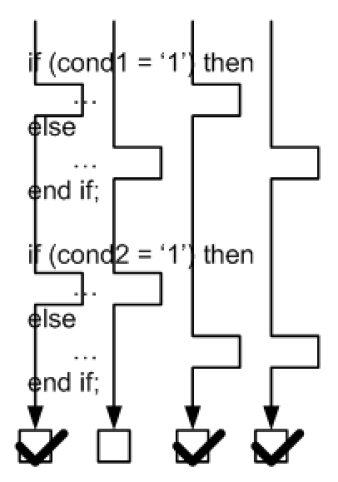
\includegraphics[scale=0.5]{img-p10-7.png}
\caption{Path Coverage Example.}
\label{img-p10-7}
\end{figure}
\paragraph{11 Condition coverage.}
\hfill \break
\indent Condition coverage beleži koliko je puta svaka permutacija članova u Bulovom izrazu izazvala da kompletan izraz ima vrednost true ili false. Razmotrimo izraz (A \&\& B) || C || D. Ovaj izraz je true u slučaju sledeća tri uslova:
\begin{enumerate}
\item A \&\& B
\item C
\item D
\end{enumerate}
a false je u slučaju ova dva uslova:
\begin{enumerate}
\item !A \&\& !C \&\& !D
\item !B \&\& !C \&\& !D
\end{enumerate}
\indent Stroža forma condition pokrivenosti - ekskluzivna condition pokrivenost - je ponekad na raspolaganju. Ona zahteva da svaki član bude kontrolišući član - da bude jedini razlog za to što izraz ima vrednost true ili false. Za gore navedeni primer izraz ima vrednost true za narednih pet ekskluzivnih uslova. Kontrolišući član je boldovan:
\begin{enumerate}
\item \textbf{A \&\& B} \&\& !C \&\& !D
\item \textbf{A} \&\& B \&\& \textbf{C} \&\& !D
\item A \&\& \textbf{!B} \&\& \textbf{C} \&\& !D
\item \textbf{!A} \&\& B \&\& !C \&\& \textbf{D}
\item A \&\& \textbf{!B} \&\& !C \&\& \textbf{D}
\end{enumerate}
\paragraph{12 FSM coverage.}
\hfill \break
\indent Moderni alati za code coverage identifikuju i izdvajaju mašine konačnog stanja iz RTLa. Postoji više FSM metrika od interesa za verifikacione inženjere:
\begin{itemize}
\item[-] Osnovna je \textbf{state coverage}: koliko puta je mašina stanja ušla u svako od stanja?
\item[-] Druga je \textbf{arc coverage}: koliko puta je FSM prešao iz jednog stanja u njemu susedna stanja? Arc coverage bi trebao da bude reportovan (reported) za pod-izraze svake jednačine narednog stanja, kao što smo videli u condition pokrivenosti.
\item[-] Treća FSM metrika je \textbf{sequential arc coverage}, često nazvana \textbf{transition coverage}. Sequential arc coverage identifikuje sekvence posete stanja različitih trajanja i beleži broj obilazaka svake sekvence.
\end{itemize}
\indent Razmotrimo primer FSMa od pet stanja i devet grana (arcs) prikazanih na slici \ref{img-state-coverage}. Pored svake grane nalazi se njoj odgovarajuća jednačina narednog stanja. Moguć izveštaj state coverage-a za ovaj FSM dat je slici pored.\\
\indent Arc coverage za isti FSM dat je na slici \ref{img-arc-coverage}.\\

\begin{figure}[h!]
\centering
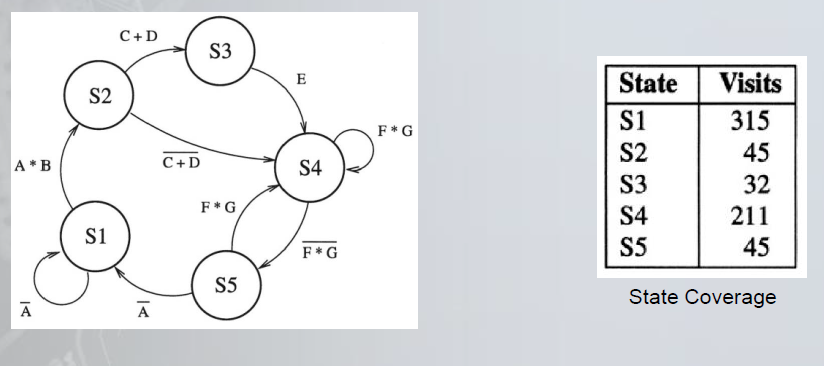
\includegraphics[scale=0.5]{img-state-coverage.png}
\caption{State Coverage.}
\label{img-state-coverage}
\end{figure}

\begin{figure}[h!]
\centering
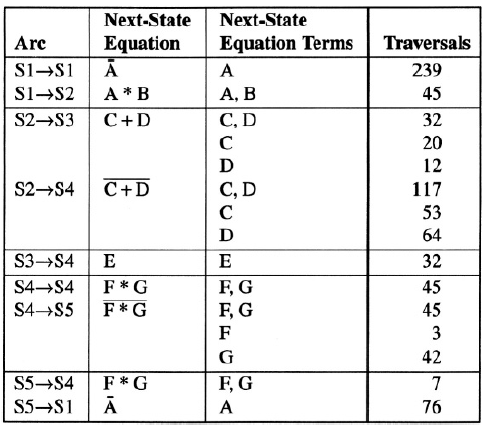
\includegraphics[scale=0.5]{img-arc-coverage.png}
\caption{Arc Coverage.}
\label{img-arc-coverage}
\end{figure}

\indent Moguć izveštaj sequential arc coverage-a za dvo-grane prelaze počevši od stanja S1, za isti FSM, dat je na slici \ref{img-sequential-arc-coverage}.

\begin{figure}[h!]
\centering
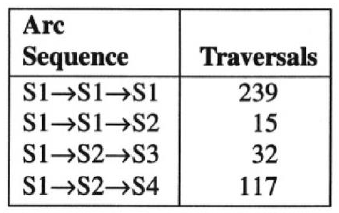
\includegraphics[scale=0.5]{img-sequential-arc-coverage.png}
\caption{Sequential Arc Coverage.}
\label{img-sequential-arc-coverage}
\end{figure}

\paragraph{13 Neophodni koraci u procesu korišćenja strukturne pokrivenosti (Code Coverage). Navesti i ukratko objasniti svaki od njih.}
\hfill \break
\indent Code coverage izveštava o tome koliko je uspešno RTL implementacija uređaja izupotrebljavana (exercised) iz perspektive ranije navedenih metrika. Pošto je RTL podložan promenama u ranim fazama dizajna, mi smo zainteresovani za izupotrebljavanost dizajna tek u kasnijim etapama dizajn ciklusa. Koraci code coverage procesa su:
\begin{itemize}
\item \textbf{instrumentacija}: Prvi korak u korišćenju strukturne (code) pokrivenosti je instrumentacija RTLa. Odabiramo module koda, hijerarhije ili instance koje ćemo posmatrati. Sledeće, odabiramo metriku koju ćemo beležiti (record). Količina instrumentovanog koda i broj merenih metrika će odrediti stepen degradacije simulacije. Moramo ograničiti ova dva faktora tako da postignemo ciljeve pokrivenosti. Poslednji korak instrumentacije zavisi od konkretnog alata koji koristimo:
\begin{itemize}
\item[-] Za započinjanje beleženja metrika neki alati ne zahtevaju dalje radnje pre simulacije.
\item[-] Drugi alati zahtevaju korak instrumentacije/kompilacije, gde u RTL ubacuju kod koji definiše brojače i inkrementira ih.
\end{itemize}
\item \textbf{beleženje metrike}: Drugi korak u primeni strukturne pokrivenosti je beleženje metrika. Ovo beleženje radi simulator tokom simulacije. Zabeleženi podaci moraju da se organizuju pre analize koja sledi. Svaka od zabeleženih metrika ima svoj prag ili hit count. Default vrednost obučno iznosi 1. U visoko rizičnim delovima RTLa, sa možda neobičnom količinom kompleksnosti, trebalo bu razmotriti povećanje praga zabeleženih metrika u ovim delovima. Ovo "over-samplovanje" će umanjiti rizik be
\item \textbf{analiza}: Treći korak u korišćenju strukturne pokrivenosti je analiziranje merenja. Irelevantni podaci moraju da se isključe iz analiza i fokus mora da bude na značenju zabeleženih metrika. Treba zapamtiti da strukturna pokrivenost ne može da otkrije potreban RTL, koji nedostaje. Ako RTL potreban za implementaciju dela funkcionalnosti uređaja nije napisan, to ne može da identifikuje strukturna pokrivenost, već samo funkcionalna. Kako bi se smanjila preopterećenost informacijama dobijenih od alata za pokrivenost koristi se data filtering.
\end{itemize}
\indent *Random useful fact: Structural coverage models have no ability to predict bugs; bug coverage model they are not.
\paragraph{14 Funkcionalna pokrivenost (Functional Coverage). Osnovna ideja.}
\hfill \break
\indent Svrha merenja funkcionalne pokrivenosti je merenje verifikacionog napretka iz perspektive funkcionalnih zahteva uređaja. Funkcionalni zahtevi za ulaze i izlaze uređaja - i njihove međusobne veze - specifikacijama uređaja (funkcionalna specifikacija i specifikacija dizajna). Zahtevi za ulaze diktiraju opseg podataka i vremenski opseg ulaznih stimulusa. Zahtevi za izlaze specificiraju potpuni skup data i temporalnih odgovora koji se posmatraju. Ulazno/izlazni zahtevi specificiraju sve stimulus/response permutacije koje se moraju posmatrati kako bi se zadovoljili black-box device zahtevi.\\
\indent Pošto ovi ulazni, izlazni i ulazno/izlazni zahtevi mogu u potpunosti da definišu ponašanje uređaja, prostor funkcionalne pokrivenosti koji oslikava ove zahteve se naziva model pokrivenosti (coverage model). Stepen u kom coverage model oslikava ove zahteve jeste njegova tačnost (fidelity). Fidelity modela određuje koliko blisko model definiše stvarne bihevijalne zahteve uređaja. Ovo je abstraction gap između modela pokrivenosti i uređaja.\\
\indent Za razliku od strukturne pokrivenosti, ne postoji automatizovan način za kreiranje modela funkcionalne pokrivenosti. Funkcionalna pokrivenost targetira semantičke aspekte test generisanja ili dizajn implementacije. Neophodno je odabrati koje funkcionalne oblasti dizajna treba testirati. Uvid u dizajn semantiku navodi ove izbore, i te uvide daju dizajner ili verifikacioni inženjeri.\\
\indent Značajna komponenta ovih uvida je znanje o kompleksnosti dizajna, za oblasti koje su sklone bugovima. Predictive bug coverage komponenta modela funkcionalne pokrivenosti potiče od iskustva inženjera. Ne postoji skup kompleksnih automatskih alata na raspolaganju za definisanje modela funkcionalne pokrivenosti. Alati većinom podržavaju implementaciju modela pokrivenosti i efikasno skupljanje podataka tokom simulacije (during runtime). Nakon što su podaci prikupljeni, alati pružaju GUI podršku za pregled rezultata.
\paragraph{15 Koraci prilikom formiranja modela funkcionalne pokrivenosti. Navesti i ukratko objasniti.}
\hfill \break
\indent Koraci prilikom formiranja modela funkcionalne pokrivenosti uključuju:
\begin{itemize}
\item opis semantike modela,
\item identifikovanje atributa (eventova) pokrivenosti i
\item specificiranje veze između ovih atributa koji karakterišu uređaj i vremena njihove korelacije. 
\end{itemize}
\indent Semantika modela je priča, opis onoga što se modeluje. Primer input coverage modela je: \textit{Dekoder instrukcija mora da dekodira svaki opkod, u svakom modu adresiranja sa svim permutacijama operand registara}. Primer output modela je: \textit{Posmatramo sekvencu paketa istog prioriteta, gde dužina sekvence varira od 1 do 255}.\\
\indent Kada je napisan opis semantike, drugi korak u dizajniranju modela pokrivenosti je identifikacija \textbf{atributa}, tj. \textbf{coverage eventova}. Šta podrazumevamo pod atributom? Atribut specificira događaj u modelu ili testbenchu, koji je dovoljno značajan da bi ga verifikaciono okruženje zapazilo i zabeležilo njegovu pojavu. Atribut identifikovan od specifikacije uređaja je parametar uređaja, poput configuration mode-a, opkoda instrukcije, vrednosti kontrolnog polja ili dužine paketa.
\paragraph{16 Matrični model zavisnosti atributa funkcionalne pokrivenosti. Objasniti i navesti primer.}
\hfill \break
\indent Matrični model razmatra svaki atribut kao dimenziju matrice, gde je broj dimenzija definisan brojem atributa. Vrednosti duž svake ose su vrednosti odgovarajućih atributa. Slika \ref{img-matrix-coverage-model} ilustruje dvodimenzionalni matrični model. Dva atributa su obeležena kao "Atribut A" i "Atribut B". Atribut A ima dvanaest vrednosti, od A0 do A11 dok atribut B ima osam vrednosti, od B0 do B7. Par atributa (An,Bm) definiše tačku u dvodimenzionalnom prostoru pokrivenosti. Ovaj matrični model definiše 96 tačaka.
\begin{figure}[h!]
\centering
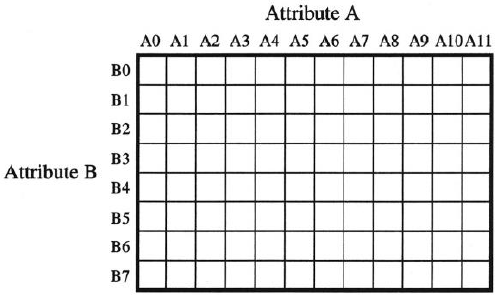
\includegraphics[scale=0.5]{img-matrix-coverage-model.png}
\caption{Matrix Coverage Model.}
\label{img-matrix-coverage-model}
\end{figure}
\paragraph{17 Hijerarhijski model zavisnosti atributa funkcionalne pokrivenosti. Objasniti i navesti primer.}
\hfill \break
\indent Hijerarhijski model ima strukturu invertovanog stabla sa korenom na vrhu. To je usmereni graf čiji su čvorovi vrednosti atributa i čije grane ukazuju na vezu između vrednosti dva atributa. Na svakom nivou stabla predstavljen je jedan atribut, sa primarnim kontrolišućim atributima u korenu stabla i svakim sukcesivnim atributom na jednom nivou niže. Slika \ref{img-hierarchical-coverage-model} ilustruje hijerarhijski model pokrivenosti definisan pomoću tri atributa: A, B i C. Atribut A je primarni kontrolišući atribut i ima 4 vrednosti, od A0 do A4. Atribut B je sekundarni atribut i ima 3 vrednosti B0, B1 i B2. Atribut C je tercijarni atribut koji ima 4 vrednosti, od C0 do C3. U ovom modelu trojka (An, Bm, Ck) definiše jednu od 10 tačaka u prostoru pokrivenosti. Npr. p7 je definisana sa (A2, B0, C2) , što je putanja do ove tačke u stablu.
\begin{figure}[h!]
\centering
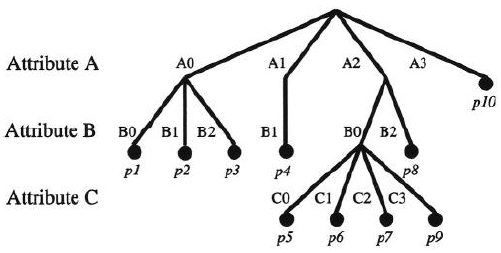
\includegraphics[scale=0.5]{img-hierarchical-coverage-model.png}
\caption{Hierarchical Coverage Model.}
\label{img-hierarchical-coverage-model}
\end{figure}

\paragraph{18 Hibridni model zavisnosti atributa funkcionalne pokrivenosti. Objasniti i navesti primer.}
\hfill \break
\indent Hibridni model je mešavina matričnih i hijerarhijskih regiona, gde su potpuno permutovane kombinacije atributa strukturirane kao matrica, a iregularne veze atributa su strukturirane hijerarhijski. Matrične podregije mogu biti listovi osnovnog hijerarhijskog modela ili hijerarhijske podregije mogu zauzimati čvorove u osnovnom matričnom modelu. Na slici \ref{img-hybrid-coverage-model} je ilustrovan hibridni model prvog tipa, gde su matrične podregije listovi osnovnog hijerarhijskog modela. Atributi A, B i C su definisani kao u prethodnom čisto hijerarhijskom modelu. Atribut D ima 3 vrednosti, D0, D1 i D2, a atribut E ima 6 vrednosti, od E0 do E5. Ova dva atributa definišu matričnu podregiju hijerarhijskog modela, dimenzija 3x2 . Na isti način atributi F i G definišu matrični podregion dimenzija 5x4. Ovaj model definiše ukupno 46 tačaka: 8 čvorova (p1, p3, p4, p5, p6, p7, p8, p9), 18 tačaka u matrici atributa  D/E i 20 tačaka u matrici atributa F/G.
\begin{figure}[h!]
\centering
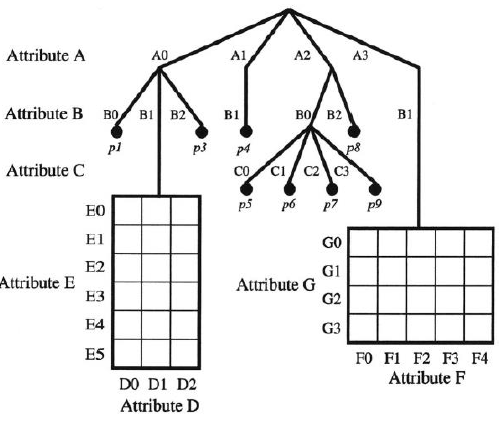
\includegraphics[scale=0.6]{img-hybrid-coverage-model.png}
\caption{Hybrid Coverage Model.}
\label{img-hybrid-coverage-model}
\end{figure}

\paragraph{19 Navesti tri modela zavisnosti atributa funkcionalne pokrivenosti. Dobre i loše strane.}
\hfill \break
\indent Iako bi struktura modela pokrivenosti trebala da oslikava vezu između atributa od kojih je model sastavljen, postoje trenuci kada veze mogu da se modeluju korišćenjem više od jedne strukture modela. koje su dobre i loše strane svake strukture u pogledu model fidelity-ja i implementacionog effort-a?\\
\indent Matrični model zahteva najmanje truda za dizajn i implementaciju zbog svoje simetričnosti. Specificira se svaki od interagujućih atributa zajedno sa njegovim odgovarajućim vrednostima. Ako je puna veličina matrično strukturiranog modela relativno mala (1.000 tačaka ili manje) i većina tačaka pokrivenosti nije ne-validno ili nedostižno, vreme sačuvano izbegavanjem dizajniranja preciznijeg hijerarhijskog ili hibridnog modela je vredno gubitka tačnosti. Ali ako bi matrični model bio značajno velik (100.000 ili više tačaka) definitivno bi imao ne-validnih tačaka, pa bi trebalo izabrati hijerarhijski ili hibridni model.\\
\indent Dizajn hijerarhijskog modela zahteva više truda jer ne samo da moramo specificirati atribute i njihove vrednosti, već moramo definisati i specifične veze između atributa. Ove veze su često iregularne i kompleksne, i njihova enumeracija zahteva velik broj linija. Ipak, kompleksnost hijerarhijskog modela je inherentno sadržana u vezama između atributa - koje su opisane specifikacijom uređaja ili RTL implementacijom. Iako se može pojednostaviti korišćenjem modela slabije tačnosti, ne može se izbeći. Jačina hijerarhijskog modela je to što može precizno da definiše veze atributa, smanjujući veličinu modela pokrivenosti i pružajući dublji uvid u ponašanje uređaja.\\
\indent U dizajn hibridnog modela je potrebno uložiti truda koliko i u hijerarhijski model. Opet, atributi, vrednosti i individualne veze se moraju enumerisati. Ipak, neki regioni hibridnog modela su regularni i predstavljeni su matričnom strukturom. Hibridni model obično najpreciznije oslikava ponašanje ulaza, izlaza ili internih uređaja, upravo zbog prirode dizajna. Oni su mešavina simetričnih vrednosti sa par ubačenih izuzetaka.
\paragraph{20 Semplovanje ulaznih atributa u slučaju funkcionalne pokrivenosti.}
\hfill \break
\indent Ulazne atribute treba da sample-uje monitor koji ima pristup primarnim ulazima u uređaj. Monitor treba da sample-uje podatke sa ulaznih signala u validnim trenucima specificiranim specifikacijom uređaja. Monitor ne bi trebao da uzima nazad svoje podatke sa stimulus generatora, jer kreiranje takve zavisnosti može da ugrozi mogućnost reuse-a monitora za beleženje pokrivenosti na sledećim nivoima integracije. Slika \ref{img-sampling-input-attributes} ilustruje sample-ovanje podataka sa primarnih ulaza u uređaj, od strane monitora. Blok obeležen sa "Coverage" je različit od "Input Monitor" bloka jer ima posebnu odgovornost dok je monitor opštije svrhe. Coverage blok je odgovoran jedino za beleženje podataka o funkcionalnoj pokrivenosti. Monitor blok je generički blok za beleženje podataka, koji se koristi i za coverage i za checking aspekte.
\begin{figure}[h!]
\centering
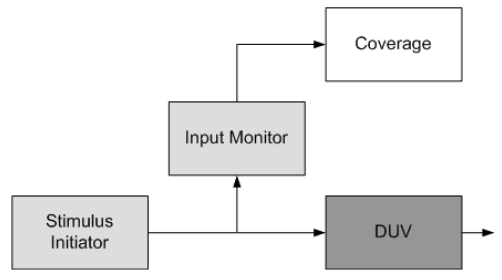
\includegraphics[scale=0.5]{img-sampling-input-attributes.png}
\caption{Sampling Input Attributes.}
\label{img-sampling-input-attributes}
\end{figure}

\paragraph{21 Semplovanje izlaznih atributa u slučaju funkcionalne pokrivenosti.}
\hfill \break
\indent Izlazne atribute bi takođe trebao da sample-uje monitor, ali naravno sa primarnih izlaza uređaja. Monitor bi trebao da sample-uje podatke u validnim trenucima specificiranim specifikacijom uređaja. Slika \ref{img-sampling-output-attributes} prikazuje sample-ovanje podataka sa primarnih izlaza uređaja, od strane monitora.
\begin{figure}[h!]
\centering
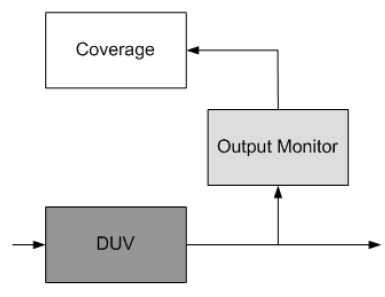
\includegraphics[scale=0.5]{img-sampling-output-attributes.png}
\caption{Sampling Output Attributes.}
\label{img-sampling-output-attributes}
\end{figure}

\paragraph{22 Semplovanje unutrašnjih atributa u slučaju funkcionalne pokrivenosti.}
\hfill \break
\indent I unutrašnji atributi uređaja imaju njima asociran monitor, odgovoran za beleženje vrednosti internih signala i registara. Za razliku od ulaznih i izlaznih interfejsa uređaja, interni signali nisi toliko dobro specificirani (ako i uopšte). Sample-ovanje takvih internih signala mora biti koordinisano sa dizajn timom kako bi se minimizovao volatility.\\
\indent Pošto interni signali mogu biti nestabilni (volatile) i često nisu specificirani, treba minimizovati korišćenje unutrašnjih atributa za model pokrivenosti. Oni nameću dodatni teret održavanja verifikacionom timu, nakon što su implementirani, jer monitor i coverage moraju kontinualno pratiti promene u dizajnu.\\
\indent Jedna strategija koja se uspešno koristi za rešavanje ovoga je definisanje skupa fiksnih signala i registara za upotrebu u verifikaciji. Verifikacioni tim identifikuje interne signale i registre neophodne za merenje pokrivenosti i dizajn tim pristane da minimizuje svoje promene. Ovaj "verifikacioni interfejs" se tretira kao intefejs eksternog uređaja, pošto je specificiran i skoro zamrznut (frozen).\\
\indent Slika \ref{img-sampling-internal-attributes} ilustruje sample-ovanje podataka sa internih signala i registara DUVa, od strane monitora.
\begin{figure}[h!]
\centering
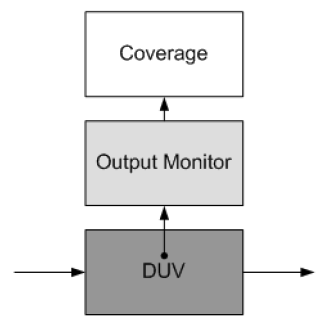
\includegraphics[scale=0.5]{img-sampling-internal-attributes.png}
\caption{Sampling Internal Attributes.}
\label{img-sampling-internal-attributes}
\end{figure}

\end{document}